\documentclass[a4paper,12pt,oneside]{report}

\usepackage[T1]{fontenc}
\usepackage[polish]{babel}
\usepackage{lmodern}        
\usepackage[babel=true]{microtype}
\usepackage[autostyle=true]{csquotes}   


\usepackage[
  a4paper,
  top=2.5cm, bottom=2.5cm,
  left=2.5cm, right=2.5cm,
  bindingoffset=1cm           % margines na oprawę (dodawany po lewej)
]{geometry}

\usepackage{setspace}
\onehalfspacing               % interlinia 1,5
\usepackage{indentfirst}      % wcięcie także w pierwszym akapicie po nagłówku


\usepackage{amsmath,amssymb}
\usepackage{booktabs}
\usepackage{tabularx}
\usepackage{array}
\usepackage{graphicx}
\graphicspath{{rysunki/}}    
\usepackage[labelsep=period,font=small]{caption}
\usepackage{enumitem}
\setlist{nosep, leftmargin=*, labelindent=\parindent}

\numberwithin{equation}{chapter}


\usepackage{titlesec}
\titleformat{\chapter}[hang]
  {\normalfont\LARGE\bfseries}{\thechapter.}{0.5em}{}
\titlespacing*{\chapter}{0pt}{0pt}{1.5em}
\titleformat{\section}
  {\normalfont\Large\bfseries}{\thesection}{0.75em}{}
\titleformat{\subsection}
  {\normalfont\large\bfseries}{\thesubsection}{0.75em}{}


\usepackage[
  backend=biber,
  style=numeric,
  sorting=none,              
  doi=true, url=false, isbn=false,
  maxbibnames=10
]{biblatex}
\addbibresource{bibliografia.bib}

\usepackage[hidelinks,unicode]{hyperref}


\newcommand{\eng}[1]{(ang.~\textit{#1})}   % np. \eng{radix sort}
\newcommand{\R}{\mathbb{R}}


\addto\captionspolish{%
  \renewcommand{\tablename}{Tabela}%
  \renewcommand{\figurename}{Rysunek}%
}


\newcommand{\uczelnia}{Uniwersytet Bielsko-Bialski}
\newcommand{\wydzial}{Wydział \dots}                % 
\newcommand{\kierunek}{\dots}                       % 
\newcommand{\autor}{Imię Nazwisko}                  % 
\newcommand{\nralbumu}{000000}                      % 
\newcommand{\promotor}{dr inż.~Imię Nazwisko}       % 
\newcommand{\tytul}{System wizualizacji i analizy scen trójwymiarowych
  metodą 3D Gaussian splatting}
\newcommand{\kategoria}{projektowa}
\newcommand{\miejscerok}{Bielsko-Biała, 2026}

\hypersetup{pdftitle={\tytul}, pdfauthor={\autor}}

\begin{document}

% !TEX root = main.tex

\begin{titlepage}
  \centering
  \singlespacing

  {\Large\scshape \uczelnia\par}
  \vspace{0.3em}
  {\large \wydzial\par}
  \vspace{0.3em}
  {\large Kierunek: \kierunek\par}

  \vspace{4cm}

  {\large Praca inżynierska\par}
  \vspace{1.5em}
  {\LARGE\bfseries \tytul\par}
  \vspace{1.5em}
  {\large Kategoria pracy: \kategoria\par}

  \vfill

  \begin{flushright}
    \begin{tabular}{@{}l@{}}
      Autor: \autor \\
      Nr albumu: \nralbumu \\[1.5em]
      Promotor: \promotor
    \end{tabular}
  \end{flushright}

  \vspace{2.5cm}

  {\large \miejscerok\par}
\end{titlepage}

\setcounter{page}{2} 

\tableofcontents
\clearpage

% !TEX root = ../main.tex
\chapter*{Wstęp}
\addcontentsline{toc}{chapter}{Wstęp}

Rekonstrukcja trójwymiarowych scen ze zdjęć jest jednym z~ważniejszych
problemów współczesnej grafiki komputerowej. Metody oparte na geometrii
wielowidokowej, takie jak Structure from Motion i~Multi-View Stereo,
dostarczały jedynie przybliżonych reprezentacji pozbawionych
fotorealistycznego wyglądu. Krokiem naprzód w~tej dziedzinie była nowa
technika neuronowych pól luminancji (NeRF), jednak jej praktyczne
zastosowanie ograniczały wielogodzinny czas treningu oraz brak możliwości
renderowania w~czasie rzeczywistym, co sprawiło, że trzeba było szukać innej
metody.

Opublikowana w~2023 roku metoda 3D Gaussian Splatting (3DGS) rozwiązuje
problemy z~treningiem i~real-time renderingiem. Reprezentuje ona scenę jako
zbiór trójwymiarowych Gaussianów i~renderuje ją za pomocą różniczkowalnego
rasteryzatora kafelkowego na GPU. Metoda ta osiąga jakość wizualną
porównywalną z~NeRF przy kilkudziesięciu klatkach na sekundę. Krótko po
publikacji 3DGS znalazł zastosowanie w~produkcji filmowej, wizualizacji
architektonicznej, a~także w~badaniach nad robotyką i~autonomicznymi
pojazdami.

Dynamiczny rozwój metody ujawnił problemy w~dostępnych narzędziach do jej
wizualizacji. Istniejące rozwiązania zmuszają użytkownika do wyboru między
narzędziami analitycznymi, narzędziami do edycji jak i~UX. Narzędzia
analityczne, jak splatviz, wymagają karty graficznej NVIDIA z~obsługą CUDA
i~oferują nieprzyjazny użytkownikowi interfejs. Narzędzia produkcyjne, jak
SuperSplat oparty na WebGL, cechują się dojrzałym UX i~możliwością edycji
scen, ale są pozbawione jakichkolwiek narzędzi do analizy scen.

Implementacje niezależne od CUDA, jak 3DGS.cpp oparte na Vulkanie, pozostają
na poziomie bazowym, bez możliwości debugowania czy przeglądania statystyk
sceny, jak i~bez możliwości edycji. Żadne z~dostępnych narzędzi nie łączy
niezależności od CUDA z~podstawową analityką, edycją i~przyjaznym UI.

Celem niniejszej pracy jest zaprojektowanie i~implementacja systemu
wizualizacji scen trójwymiarowych opartego na metodzie 3DGS, działającego
niezależnie od technologii CUDA, z~wykorzystaniem języka C++, graficznego
API OpenGL i~wprowadzonych w~wersji 4.3 OpenGL-a compute shaderów.

Praca ta obejmuje analizę istniejących rozwiązań, implementację całego
potoku graficznego -- od wczytywania splatów do rasteryzacji Gaussianów --
oraz testy wydajnościowe.

% !TEX root = ../main.tex
\chapter{Rys historyczny i aktualny stan wiedzy}
\label{chap:stan-wiedzy}


\section{Historia rekonstrukcji scen trójwymiarowych}
\label{sec:historia}

Rekonstrukcja scen trójwymiarowych jest jednym z~problemów współczesnej wizji
komputerowej. Problem polega na odtworzeniu głębi z~płaskich zdjęć.
Zazwyczaj głębia ta jest tracona w~wyniku projekcji perspektywicznej.
Ewolucja tej dziedziny prowadzi nas od matematycznej fotogrametrii, przez
statystyczne dopasowywanie cech, aż po rewolucję, jaką przyniosło nam głębokie
uczenie maszynowe.

Podstawy rekonstrukcji scen 3D sięgają XIX wieku i~są związane
z~fotogrametrią. Fotogrametria to nauka zajmująca się określaniem kształtów
i~położeń obiektów na podstawie dostępnych zdjęć. Przed erą komputerów proces
ten opierał się na ręcznej identyfikacji punktów wspólnych na zdjęciach.
Automatyzacja nastąpiła wraz ze sformułowaniem matematycznych podstaw geometrii
wielowidokowej. Metody opracowane w~tym czasie pozwoliły powiązać ze sobą
punkty na różnych obrazach przedstawiających tę samą scenę.

Wczesne komputery nie posiadały jednak stabilnych metod automatycznego
znajdowania punktów wspólnych na zdjęciach. Kluczowa okazała się praca
Davida Lowe'a, która zaprezentowała algorytm SIFT \eng{Scale-Invariant Feature
Transform}~\cite{lowe2004sift}. Algorytm ten pozwolił na identyfikację punktów
charakterystycznych na obrazach w~sposób odporny na zmiany związane ze skalą
i~rotacją, a~także na częściowe zmiany oświetlenia i~perspektywy.

Połączenie deskryptorów lokalnych z~algorytmami, które były odporne na szum,
sprawiło, że można było stworzyć pierwsze w~pełni automatyczne systemy potoku SfM
\eng{Structure from Motion}. Photo Tourism~\cite{snavely2006phototourism} było
platformą, która pokazała, że możliwe jest zrekonstruowanie rzadkiej chmury
punktów oraz pozycji kamer z~tysięcy nieuporządkowanych zdjęć pobranych
z~internetu. Problem jednak polegał na tym, że SfM generowało wyłącznie rzadkie
chmury punktów, które, chociaż opisywały geometrię sceny z~perspektywy kamer,
były zbyt ubogie dla zastosowań wizualizacyjnych (VR, geologia). Rozwiązaniem
miało być opracowanie algorytmów MVS \eng{Multi-View Stereo}, które potrafiły
zagęścić chmurę punktów. Następnym krokiem była zamiana punktów na siatki
wielokątów. Połączenie SfM i~MVS było branżowym standardem. Metody te miały
jednak jedną dużą wadę: nie radziły sobie z~powierzchniami bezteksturowymi,
błyszczącymi, przezroczystymi czy zawierającymi powtarzalne wzory.

Powiew świeżości nastąpił w~2020 roku, kiedy zaczęły pojawiać się prace nad
NeRF \eng{Neural Radiance Fields}~\cite{mildenhall2020nerf}. Zamiast traktować
przestrzeń jako punkty czy trójkąty, badacze zaproponowali potraktowanie sceny
jako ciągłego pola funkcji, które jest reprezentowane przez głęboką sieć
neuronową (MLP). Chociaż NeRF zachwycał fotorealizmem, był bardzo kosztowny
obliczeniowo. To doprowadziło do narodzin 3D Gaussian Splatting
(3DGS)~\cite{kerbl2023gaussian}. Metoda ta łączyła zalety reprezentacji
jawnych i~ciągłych pól luminancji.


\section{Wprowadzenie do metody 3DGS}
\label{sec:3dgs}

\subsection{Reprezentacja sceny}
\label{subsec:reprezentacja}

Zaprezentowana w~2023 roku w~pracy~\cite{kerbl2023gaussian} metoda
3D Gaussian Splatting rozwiązywała praktycznie wszystkie problemy technologii
NeRF. Metoda ta porzuciła koncepcję ciągłego reprezentowania sceny przez sieć
MLP na rzecz reprezentacji za pomocą trójwymiarowych elipsoid Gaussa (splatów).
Scena składa się z~punktów, które stają się elipsoidami opisanymi przez zestaw
parametrów:
\begin{enumerate}
  \item Pozycja (środek): wektor $X = (x, y, z)$ określający punkt będący
        środkiem Gaussiana.
  \item Skala (wymiary): wektor $S = (s_x, s_y, s_z)$.
  \item Rotacja: reprezentowana przez kwaternion $Q = (q_w, q_x, q_y, q_z)$
        w~celu uniknięcia blokady przegubu.
  \item Nieprzezroczystość: wartość $\alpha \in [0, 1]$.
  \item Kolor zależny od kierunku: zestaw współczynników harmonik sferycznych,
        który pozwala na zmianę koloru elipsoidy w~zależności od kierunku.
\end{enumerate}

Kształt i~orientację Gaussiana opisuje macierz kowariancji
$\Sigma \in \R^{3 \times 3}$. Macierz ta musi być dodatnio określona, aby
zapewnić geometryczny sens, dlatego stosuje się następującą postać:
\begin{equation}
  \Sigma = R\,S\,S^{\top} R^{\top}.
  \label{eq:kowariancja}
\end{equation}
Macierz $R \in \mathrm{SO}(3)$ jest macierzą rotacji wyznaczaną z~kwaternionu
jednostkowego $Q$, a~$S$ jest macierzą diagonalną, która na przekątnej zawiera
wartości skali.

Popularnym formatem plików do przechowywania informacji o~Gaussianach jest
format PLY. Wartość skali jest w~nim przechowywana po zlogarytmowaniu, co
sprawia, że podczas odczytu z~pliku należy zastosować funkcję wykładniczą.
Nieprzezroczystość jest w~tym formacie przechowywana jako logit, zgodnie ze
wzorem:
\begin{equation}
  \alpha = \sigma(x) = \frac{1}{1 + \exp(-x)}.
  \label{eq:sigmoid}
\end{equation}
Kolor natomiast jest modelowany za pomocą harmonik sferycznych (SH) stopnia~3.
Wymaga to 16 współczynników SH dla każdego kanału RGB, co daje łącznie
48~wartości.

\subsection{Projekcja Gaussianów na ekran}
\label{subsec:projekcja}

Renderowanie sceny odbywa się poprzez rzutowanie trójwymiarowych Gaussianów
na ekran i~ich kompozytowanie. Podstawy tej operacji wywodzą się
z~pracy~\cite{zwicker2002ewa}, która zaprezentowała metodę EWA Splatting
\eng{Elliptical Weighted Average Splatting}.

Oznaczmy przez $W$ macierz transformacji widoku, która przekształca punkt
z~przestrzeni sceny do przestrzeni kamery. Projekcja perspektywiczna jest
przekształceniem nieliniowym, co uniemożliwia zastosowanie jej do Gaussianów.
Wykorzystuje się zatem jakobian $J$ do odwzorowania projekcji w~punkcie, który
jest reprezentowany przez wektor pozycji $X$. Macierz kowariancji Gaussiana
w~przestrzeni 2D przyjmuje postać:
\begin{equation}
  \Sigma' = J\,W\,\Sigma\,W^{\top} J^{\top}.
  \label{eq:kowariancja2d}
\end{equation}

Do obliczeń wykorzystuje się tylko górną lewą podmacierz macierzy $\Sigma'$.
Wtedy potrzebną nam macierz $2 \times 2$ możemy przedstawić jako
\begin{equation}
  \Sigma'_2 =
  \begin{bmatrix}
    a & b \\
    b & c
  \end{bmatrix},
  \label{eq:kowariancja2x2}
\end{equation}
gdzie $a$, $b$, $c$ to elementy macierzy kowariancji w~2D. Macierz ta
definiuje elipsę, której osie wyznaczone są przez wektory i~wartości własne
$\lambda_1$ i~$\lambda_2$ (służą do wyznaczania \textit{bounding box} dla
rasteryzatora). Przekształcenie to odpowiada rzutowi trójwymiarowego Gaussiana
na płaszczyznę ekranu z~uwzględnieniem perspektywy kamery.

\subsection{Renderowanie i sortowanie}
\label{subsec:renderowanie}

Finalna barwa piksela wyznaczana jest metodą \textit{alpha compositing}.
Oznacza to przetwarzanie Gaussianów w~kolejności od najdalszego do
najbliższego kamery. Kolor każdego piksela jest obliczany zgodnie
z~równaniem:
\begin{equation}
  C(p) = \sum_{i} c_i\, \alpha_i(p) \prod_{j<i} \bigl(1 - \alpha_j(p)\bigr).
  \label{eq:compositing}
\end{equation}
% TODO: iloczyn po j<i we wzorze (eq:compositing) odpowiada kolejności
% front-to-back (i = 1 to Gaussian NAJBLIŻSZY kamery). Tekst wyżej i niżej
% mówi o kolejności od najdalszego i numeracji malejąco wg głębokości —
% ujednolicić opis ze wzorem.
Indeks $i$ numeruje Gaussiany malejąco według głębokości \eng{depth}.
$c_i$ jest kolorem $i$-tego Gaussiana wyznaczonym przez SH dla bieżącego
kierunku patrzenia. Nieprzezroczystość $\alpha_i$ jest liczona w~zależności od
odległości piksela od centrum elipsy:
\begin{equation}
  \alpha_i(p) = o_i \exp\!\left(-\tfrac{1}{2}\, d^{\top} \left(\Sigma'_2\right)^{-1} d\right),
  \label{eq:alpha}
\end{equation}
% TODO: dopisać, czym jest o_i (nieprzezroczystość Gaussiana z p. 1.2.1)
% i mu'_2 (rzutowany środek Gaussiana).
gdzie $d = p - \mu'_2$ jest wektorem przesunięcia piksela od rzutowanego
centrum Gaussiana.

Sortowanie stanowi największe wyzwanie, jeśli chodzi o~wydajność metody.
Sortowanie na CPU może okazać się za mało efektywne, gdyż sceny potrafią
posiadać ponad 1~mln Gaussianów. Żeby rozwiązać ten problem, często stosuje się
algorytmy równoległe do sortowania na karcie graficznej. Najczęściej stosowane
jest sortowanie pozycyjne \eng{radix sort}. Implementacja sortowania
pozycyjnego na GPU pozwala zredukować czas sortowania miliona Gaussianów do
kilku milisekund, podczas gdy analogiczna operacja na CPU zajmuje czas rzędu
dziesiątek milisekund.

\subsection{Trening}
\label{subsec:trening}

Inicjalizacja zbioru Gaussianów zaczyna się od metody SfM, która generuje
rzadkie chmury punktów z~tych samych zdjęć użytych do treningu. Każdy punkt
chmury staje się środkiem jednego Gaussiana z~kulistą kowariancją i~losową
barwą SH.


Proces treningu minimalizuje funkcję straty, porównując obrazy wyrenderowane
ze zdjęciami ze zbioru treningowego. Funkcja straty to kombinacja błędu L1
i~miary strukturalnej D-SSIM.

Ważnym elementem treningu jest kontrola gęstości Gaussianów. Algorytm co pewną
liczbę iteracji dokonuje zagęszczania i~przycinania. Proces ten klonuje lub
dzieli Gaussiany o~dużym gradiencie pozycji, a~także usuwa Gaussiany o~małym
rozmiarze, niskiej nieprzezroczystości. Pozwala to na automatyczne
dostosowanie liczby i~rozmieszczenia Gaussianów w~zależności od sceny.

\section{Analiza istniejących rozwiązań}
\label{sec:analiza}

Istnieje wiele narzędzi, które umożliwiają wizualizację, edycję i~analizę
sceny za pomocą metody 3DGS. Rozwiązania te można podzielić na aplikacje
desktopowe wymagające CUDA, aplikacje webowe oraz implementacje oparte na
otwartych standardach i~bibliotekach graficznych. Poniżej omówiono trzy
reprezentatywne narzędzia.

\subsection{splatviz}
\label{subsec:splatviz}

Splatviz to narzędzie autorstwa Floriana Barthela. Jest to aplikacja
desktopowa napisana w~Pythonie, renderująca sceny 3DGS za pomocą kerneli CUDA
i~wyświetlająca interfejs za pomocą biblioteki ImGui osadzonej w~oknie OpenGL.
Każda funkcja analityczna to osobny widget UI.

Możliwości renderowania wykraczają poza standardowe narzędzia. Aplikacja ta
obsługuje tryb split-screen, co pozwala na porównanie wizualne między różnymi
metodami treningowymi lub parametrami. Są dostępne tryby debugowania, które
pokazują kanał głębokości i~alpha.

Tym, co wyróżnia splatviz, jest warstwa analityczna. Widget Evaluate pozwala
na wpisanie kodu w~Pythonie, który jest wykonywany po renderingu i~daje dostęp
do zmieniania kontekstu renderowania oraz wizualizacji zmian w~postaci
histogramów. Widget Edit pozwala na zmianę zbioru Gaussianów przez kod
w~Pythonie, co umożliwia filtrowanie według pewnych kryteriów.

Ograniczeniem tego rozwiązania jest konieczność kompilacji na urządzeniach
wspierających CUDA, co wyklucza użytkowników nieposiadających kart GPU NVIDIA.

\subsection{SuperSplat}
\label{subsec:supersplat}

SuperSplat firmy PlayCanvas to aplikacja webowa oparta na WebGL~2.0. Sprawia
to, że viewer ten działa w~przeglądarce bez instalacji. Jest to standard
branżowy w~zakresie prezentacji i~edycji scen 3DGS.

Rozwiązanie to posiada wiele funkcji edycyjnych: narzędzia do selekcji
i~usuwania Gaussianów, kompresję sceny i~kadrowanie obszaru roboczego oraz
eksport do formatów PLY lub SPLAT. Zawiera też wbudowaną historię zmian
z~funkcją cofania ostatnich zmian. Mamy też efekty post-processingu, wsparcie
WebXR, co pozwala na oglądanie scen na urządzeniach VR/AR, a~także do 25
adnotowanych hotspotów z~tytułami, opisami i~zapisanymi widokami kamery.
Funkcja Timeline pozwala na tworzenie animowanych przelotów przez scenę.

Tym, czego na pewno brakuje SuperSplat, są funkcje analityczne. Edytor
wyświetla histogramy podstawowych właściwości i~podstawowe statystyki
numeryczne sceny, ale nie posiada narzędzi analizy ani dostępu do parametrów
Gaussianów, które pozwalałyby na własne metryki jakości. Ograniczenia te
wynikają z~tego, że rozwiązanie to bazuje na WebGL~2.0, co utrudnia eksport
danych do warstwy analitycznej.

\subsection{3DGS.cpp}
\label{subsec:3dgscpp}

Projekt 3DGS.cpp autorstwa shg8 wykorzystuje Vulkan API i~compute pipeline.
Vulkan został wybrany ze względu na dostępność prymitywów warp-level zbliżonych
do CUDA. W~obecnej wersji API OpenGL jest uznawany za przestarzały na
platformach Apple. Obsługiwane platformy to Windows, Linux, macOS, iOS
i~visionOS.

Jest to aplikacja C++ z~modułową strukturą oddzielającą backend renderujący od
warstwy okienkowej. Shadery Vulkana (SPIR-V) implementują kolejne etapy
potoku: preprocessing Gaussianów, sortowanie pozycyjne na GPU i~rasteryzację.
Funkcje wizualizacyjne to m.in.\ kontrola kamery, ładowanie pliku PLY
i~podstawowe parametry renderowania.

Największa wartość rozwiązania polega na demonstracji tego, że można stworzyć
viewer, nie używając do tego CUDA, a~używając otwartych standardów. Projekt
udowadnia, że wydajność, którą zapewniają karty NVIDIA, jest osiągalna na
kartach AMD, Intel i~Apple Silicon, co rozszerza grupę odbiorców. Brakuje tutaj
natomiast funkcji analitycznych, edycyjnych i~trwałych operacji zapisu.

\subsection{Zestawienie i wnioski}
\label{subsec:zestawienie}

Tabela~\ref{tab:porownanie} zawiera zestawienie porównawcze omówionych
narzędzi według wybranych kryteriów funkcjonalnych i~technologicznych.

\begin{table}[htbp]
  \centering
  \caption{Zestawienie porównawcze narzędzi wizualizacji scen 3DGS}
  \label{tab:porownanie}
  \small
  \renewcommand{\arraystretch}{1.2}
  \begin{tabularx}{\textwidth}{
      >{\raggedright\arraybackslash}p{0.2\textwidth}
      >{\raggedright\arraybackslash}X
      >{\raggedright\arraybackslash}X
      >{\raggedright\arraybackslash}X}
    \toprule
    \textbf{Kryterium} & \textbf{splatviz} & \textbf{SuperSplat} & \textbf{3DGS.cpp} \\
    \midrule
    Stos technologiczny & Python + CUDA + ImGui & Web (PlayCanvas / WebGL~2) & C++ + Vulkan \\
    Platforma           & Linux/Win (NVIDIA) & Przeglądarka (uniwersalna) & Win/\allowbreak Linux/\allowbreak macOS/\allowbreak iOS \\
    Wizualizacja        & Zaawansowana (multi-scene, debug) & Dojrzała + WebXR & Bazowa \\
    Analityka           & Bardzo silna (Eval Widget, histogramy) & Podstawowa & Brak \\
    Edycja              & Minimalna (przez kod) & Bardzo silna (selekcje, timeline) & Brak \\
    Format wejściowy    & .ply, .yml & .ply, .splat, .ksplat, .sogs & .ply \\
    Zależność od CUDA   & Tak & Nie & Nie \\
    \bottomrule
  \end{tabularx}
\end{table}

Proponowany w~pracy viewer 3DGS będzie stworzony w~języku C++ z~użyciem
OpenGL. Będzie to rozwiązanie niewymagające CUDA, posiadające ergonomię
interfejsu oraz podstawowe narzędzia do analizy. W~potoku realizacji
zastosowane będą compute shadery (dostępne od OpenGL~4.3), żeby
zaimplementować sortowanie pozycyjne.

\chapter{Technologie i narzędzia}
\label{chap:technologie}
Wybrane technologie i narzędzia miały za zadanie zrealizować wymagania projektu jak wieloplatformowość, niezależność od CUDA, czas rzeczywisty dla scen rzędu milionów Gaussianów, jak i stworzyć warstwę interfejsu i analizy. Takie wymagania sprawiają, że nie jesteśmy uzależnieni od kart NVIDIA, zostają wykluczone języki interpretowane w warstwie renderującej i musi istnieć GUI potrzebne do analizy.
\section{Język C++ (standard C++20)}
\label{sec:c++}
C++ to wszechstronny kompilowany język programowania ogólnego przeznaczenia. Powstał jako rozszerzenie języka C o mechanizmy programowania obiektowego, umożliwia abstrakcję danych oraz stosowanie kilku paradygmatów programowania: proceduralnego, obiektowego, generycznego, modularnego i funkcjonalnego. Język ten został wybrany ze względu na ręczne zarządzanie pamięcią i zerowy narzut abstrakcji. Wizualizacja scen 3DGS wymaga przetwarzania milionów splatów w każdej klatce, a każda warstwa pomiędzy kodem a sterownikiem graficznym przekłada się na wolniejsze wykonywanie kodu źródłowego. C++ zapewnia pełną kontrolę nad układem danych w pamięci, co pomaga przygotować dane do wysłania na GPU bez kosztownych konwersji. Z mechanizmów standardu C++20 wykorzystano \texttt{std::bit\_cast} z nagłówka \texttt{<bit>}, użyty przy budowie kluczy sortowania po głębokości~\cite{wg21_2020draft}. Porównywane jest sortowanie na GPU z sortowaniem równoległym na CPU (\texttt{std::execution::par\_unseq}, mechanizm wprowadzony w C++17). Język ten jest popularny w środowisku grafiki komputerowej -- API graficzne i biblioteki matematyczne udostępniają interfejsy w C lub C++.
\section{OpenGL 4.3 Core Profile}
\label{sec: opengl}
OpenGL to otwarta, wieloplatformowa i uniwersalna specyfikacja do tworzenia grafiki 3D, rozwijana przez Khronos Group. Podstawową cechą OpenGL jest to, że jest on tzw. maszyną stanu \eng{state machine}. Na stan w danej chwili składają się parametry i tryby działania ustawiane wywołaniami funkcji; raz ustawiona wartość obowiązuje aż do jej zmiany i wpływa na wynik renderowania. W projekcie wykorzystano wersję 4.3 Core, co pozwala wykorzystać shadery obliczeniowe \eng{compute shaders} oraz Shader Storage Buffer Object, czyli bufory pozwalające na zapis i odczyt dużych struktur danych z poziomu shadera~\cite{khronos2013opengl43}. Te dwa mechanizmy pozwalają zaimplementować potok renderowania 3DGS bez użycia CUDA. Rozważaną alternatywą dla OpenGL było inne API grupy Khronos: Vulkan. Vulkan został użyty m.in.\ w 3DGS.cpp, oferując jawną kontrolę nad pamięcią oraz dostęp do operacji na poziomie podgrup. To API jednak wymaga bardzo złożonej i rozbudowanej warstwy inicjalizacyjnej, co pochłonęłoby o wiele więcej czasu niż implementacja w OpenGL. OpenGL zatem został wybrany, gdyż jest wspierany przez sterowniki wszystkich głównych producentów GPU, jest wieloplatformowy (aczkolwiek w obecnej wersji API OpenGL jest uznawany za przestarzały na platformach Apple) i udostępnia wszystkie mechanizmy potrzebne do metody 3DGS.
\section{GLFW 3.4}
\label{glfw}
GLFW to lekka, otwartoźródłowa biblioteka napisana w C, odpowiadająca za okno aplikacji, kontekst w OpenGL czy obsługę urządzeń wejściowych~\cite{glfw34docs}. Jest wykorzystywana do ukrycia różnic między systemami operacyjnymi i ich systemami okienkowymi (Win32, X11, Wayland, Cocoa). Biblioteka zawiera również precyzyjny zegar systemowy użyty do pomiaru czasu klatki. Kolejną zaletą jest integracja z biblioteką Dear ImGui, dostarczona w postaci gotowego backendu. Bez niej zdarzenia trzeba byłoby przekazywać do interfejsu użytkownika ręcznie. Wersja 3.4 wprowadziła stabilne wsparcie dla protokołu Wayland, co ma znaczenie przy uruchamianiu aplikacji na współczesnych dystrybucjach Linuksa. Alternatywą była biblioteka SDL, która obejmuje szerszy zakres funkcji, obsługę dźwięku i kontrolerów. Ponieważ aplikacja nie wymaga warstwy audio, przewaga ta nie ma znaczenia, a mniejszy rozmiar przemawia na korzyść GLFW.
\section{GLAD 2}
\label{glad}
OpenGL definiuje jedynie interfejs funkcji, natomiast ich implementacja znajduje się w sterowniku karty graficznej i nie jest dostępna w postaci statycznie linkowanej biblioteki. Adresy funkcji muszą zostać pobrane za pośrednictwem mechanizmów systemowych, co wymuszałoby na programiście ręczne pozyskanie kilkuset wskaźników. GLAD tworzy loader na podstawie przekazanej wersji API oraz profilu~\cite{glad2repo}. Loader to kod źródłowy deklarujący i inicjalizujący wyłącznie te funkcje, które są potrzebne. W projekcie wykorzystano GLAD w wersji 2 generujący loader dla konfiguracji 4.3 bezpośrednio na etapie konfiguracji. Dzięki temu wygenerowany kod nie jest przechowywany w repozytorium, lecz powstaje automatycznie podczas budowania. Profil Core zapewnia korzyść w postaci wczesnego wykrywania błędów. Próba użycia funkcji usuniętej z profilu Core (co znaczy, że funkcja pochodziła z przestarzałego potoku stałofunkcyjnego) zakończy się błędem kompilacji. Alternatywą mogłaby być biblioteka GLEW, jednak ładuje ona pełen zestaw rozszerzeń niezależnie od potrzeb aplikacji. GLAD 2 ma również opcję generowania powtarzalnego wyniku, co jest ważne przy weryfikacji, że kolejne kompilacje projektu dają te same artefakty.
\section{GLM (OpenGL Mathematics)}
\label{glm}
GLM to biblioteka nagłówkowa napisana w C++, której typy mają wiernie odwzorowywać typy występujące w języku GLSL~\cite{glmrepo}. Biblioteka ta nie jest ograniczona tylko do funkcji znajdujących się w GLSL, ale jest rozszerzona o mechanizmy związane z przekształceniami macierzy, generowaniem liczb losowych i szumem. GLM przechowuje macierze w postaci kolumnowej, zgodnie z konwencją przyjętą w OpenGL, dzięki czemu można je przesyłać bez transpozycji. W projekcie biblioteka ta została użyta do wyznaczenia macierzy projekcji perspektywicznej, widoku, przekształceń kamery oraz do normalizacji wektorów. Biblioteka, będąc biblioteką nagłówkową, nie wymaga osobnego kompilowania ani linkowania, co przyspiesza integrację. Funkcje szablonowe są w pełni rozwijane w miejscu wywołania i podlegają optymalizacji kompilatora.
\section{Dear ImGui 1.91.8}
\label{imgui}
Dear ImGui to popularna biblioteka używana do tworzenia interfejsu użytkownika. Działa w tzw. immediate mode: kontrolki nie są trwałymi obiektami o własnym stanie, lecz są deklarowane od nowa w każdej klatce jako wywołania funkcji zwracające informację o interakcji użytkownika~\cite{imgui1918repo}. Dzięki takiemu podejściu znika konieczność synchronizowania stanu interfejsu ze stanem aplikacji. Jest to przydatne w aplikacji, w której parametry renderowania zmieniają się nieustannie. Biblioteka renderuje warstwę graficzną przy użyciu tego samego kontekstu OpenGL co scena, przez co nie wprowadza dodatkowych zależności systemowych i nie wpływa na wieloplatformowość aplikacji. Integrację zapewniają backendy GLFW i OpenGL 3, które przejmują obsługę zdarzeń wejściowych i wystawianie list rysowania. W tym projekcie ImGui odpowiada za panel sterowania parametrami renderowania, prezentację statystyk i przełączanie trybów renderowania. Interfejs jest kluczową przewagą nad narzędziem 3DGS.cpp, które udostępnia niewielką liczbę opcji konfiguracyjnych. Biblioteka jest mało wymagająca obliczeniowo, a jej narzut pamięciowy nie zależy od liczby splatów. Alternatywą dla Dear ImGui jest Qt, które oferuje bogatszy zestaw kontrolek, kosztem większej zależności zewnętrznej, bardziej złożonego procesu budowania i konieczności utrzymywania osobnej reprezentacji stanu interfejsu.
\section{ImPlot 1.0}
\label{implot}
ImPlot to biblioteka do wizualizacji wykresów stworzona na bazie Dear ImGui, dziedzicząca immediate mode oraz sposób integracji z aplikacją~\cite{implotrepo}. W projekcie odpowiada za warstwę analityczną. Za jej pomocą prezentowane są rozkłady nieprzezroczystości oraz skali Gaussianów, które są obecnie widoczne, a także histogram rozmiaru rzutowanych elips w przestrzeni ekranu. Dzięki tym informacjom można przeprowadzić analizę sceny -- na przykład rozpoznać nadmiar splatów o niskiej nieprzezroczystości, które spowalniają rendering. Wykresy reagują na ruch kamery i mogą służyć do analizy poszczególnych fragmentów sceny (co jest dodatkowo możliwe poprzez zapisanie ustawień kamery w pliku .json). ImPlot został jeszcze wykorzystany do zebrania pomiarów wydajnościowych przy różnych rodzajach sortowania splatów po głębokości. Rozwiązaniem alternatywnym byłby eksport danych do pliku i analiza ich w zewnętrznym narzędziu, co uniemożliwiałoby obserwację rozkładów w czasie rzeczywistym.
\section{Happly}
\label{happly}
W programie splat jest reprezentowany przez strukturę w kodzie. Sceny 3DGS są zapisywane w formacie .ply opracowanym na Uniwersytecie Stanforda. Format jest zbudowany z nagłówka deklarującego tekstowo elementy, ich właściwości i typy, jak i z danych właściwych, zapisanych w postaci tekstowej albo binarnej. W przypadku 3DGS na element vertex składa się kilkadziesiąt właściwości, takich jak pozycja, skala, kwaternion rotacji, nieprzezroczystość oraz współczynniki harmonik sferycznych. Ze względu na dużą liczbę rekordów często te pliki mają rozmiar setek megabajtów. Happly to nagłówkowa biblioteka udostępniająca ten format w postaci prostego interfejsu opartego na pobieraniu nazwanych parametrów wskazanego elementu~\cite{happlyrepo}. W projekcie została opakowana funkcją pomocniczą sprawdzającą, czy dana własność występuje. Dzięki temu można obsłużyć pliki pochodzące z różnych implementacji treningu lub różniące się liczbą zapisanych harmonik sferycznych. Cechą, która na to pozwala, jest samoopisywalność formatu PLY: z nagłówka można odczytać, jakie właściwości są w pliku. Dane odczytane z pliku zostają przetworzone przed zapisaniem ich do struktury splatu (np.\ funkcja sigmoidalna na nieprzezroczystości, funkcja wykładnicza na skali, normalizacja kwaternionu). Ta biblioteka została wybrana ze względu na łatwą integrację i brak zależności zewnętrznych. Alternatywą była biblioteka tinyply, która oferowała zbliżoną funkcjonalność, ale o bardziej rozbudowanym interfejsie, opartym na jawnym zarządzaniu buforami.
\section{Biblioteki pomocnicze}
\label{help_lib}
\subsection{stb}
\label{stb}
stb to zbiór jednoplikowych bibliotek nagłówkowych upowszechniony przez Seana Barretta. W projekcie wykorzystano dwa moduły: stb\_image\_write do zapisu zrzutu ekranu do pliku PNG oraz stb\_image do wczytywania obrazów (wykorzystywane przy prototypowaniu)~\cite{stbrepo}. Zaletą bibliotek stb jest brak jakichkolwiek zależności i licencja nienakładająca ograniczeń, a koszt integracji sprowadza się do dołączenia do projektu pojedynczego pliku nagłówkowego.
\subsection{nlohmann/json 3.11.3}
\label{json}
Biblioteka ta pozwala na obsługę formatu JSON w postaci interfejsu zbliżonego do kontenerów biblioteki standardowej~\cite{nlohmannJsonDocs}. W projekcie służy do zapisu i odczytu ustawień kamery oraz ścieżek przejazdów w testach wydajnościowych. Dzięki formatowi tekstowemu pliki konfiguracyjne pozostają czytelne i edytowalne poza aplikacją, co ułatwia ich przygotowanie do powtarzalnych scenariuszy pomiarowych. Zapis ustawień umożliwia porównanie wydajnościowe pomiędzy kolejnymi iteracjami implementacji.
\subsection{nativefiledialog-extended 1.2.1}
\label{filedialog}
Biblioteka ta udostępnia interfejs do otwierania systemowych okien wyboru pliku, wywołując pod spodem natywne mechanizmy danej platformy~\cite{nativefiledialogRepo}. Dzięki temu użytkownik korzysta z okna dialogowego występującego w jego środowisku, zamiast z implementacji przygotowanej wewnątrz aplikacji.

\section{CMake}
\label{cmake}
CMake to wieloplatformowe narzędzie służące do zarządzania procesem budowania aplikacji, które na podstawie opisu projektu generuje pliki dla natywnego narzędzia budującego danej platformy. Rozwiązanie to jest standardem w projektach C++ dzięki przenośności, ponieważ pozwala utrzymać jeden opis projektu dla wielu platform jednocześnie. Wymagana wersja CMake to 3.21, a dzięki FetchContent wszystkie zależności zewnętrzne są pobierane automatycznie poprzez klonowanie wskazanych repozytoriów~\cite{cmake320fetchcontent}. Dla każdej zależności została zadeklarowana konkretna wersja, co sprawia, że proces budowania jest powtarzalny i odporny na zmiany wprowadzone w repozytoriach źródłowych. Dzięki takiemu podejściu nie ma potrzeby przechowywania kodu bibliotek ani ręcznego instalowania wymaganych zależności. CMake pozwala również na kopiowanie po zakończonej kompilacji plików takich jak shadery i zasoby do katalogu wynikowego, dzięki czemu nie trzeba dodatkowo przygotowywać środowiska.
% !TEX root = ../main.tex
\chapter{Projekt systemu}
\label{chap:projekt_systemu}
Rozdział 2 opisywał narzędzia, z których został zbudowany system. Ten rozdział odpowie na pytanie, jak został zaprojektowany ten system: definiuje zakres systemu, wymagania funkcjonalne i pozafunkcjonalne, strukturę, model danych i przebieg potoku renderowania. Szczegóły implementacyjne (kod, shadery, struktury pomocnicze) omówiono w rozdziale czwartym, a analizę i weryfikację w rozdziale piątym.

\section{Założenia i zakres systemu}
\label{sec:zalozenia}
Dzięki analizie istniejących rozwiązań (tabela \ref{tab:porownanie}) wynika, że żadna implementacja nie łączy jednocześnie trzech cech: niezależności od CUDA, warstwy analitycznej i interfejsu, który nie wymaga od użytkownika modyfikowania kodu. Zaprojektowany system wypełnia tę lukę.
\begin{enumerate}
    \item System służy do przeglądania wytrenowanej sceny 3DGS, a nie jest narzędziem do trenowania. Jako wejście przyjmuje gotowy plik \texttt{.ply}, wytworzony przez zewnętrzny model.
    \item Cały potok potrzebny do renderowania sceny korzysta wyłącznie z mechanizmów OpenGL 4.3 Core, bez dodatkowych zależności od bibliotek producenta kart graficznych.
    \item Obraz musi powstać w czasie rzeczywistym, a zmiana parametrów renderowania musi być widoczna natychmiast bez ponownego wczytania sceny.
    \item Każda funkcja analityczna jest dostępna z poziomu interfejsu graficznego. Użytkownik nie edytuje plików konfiguracyjnych ani kodu źródłowego.
    \item System musi umożliwiać powtarzalny pomiar wydajności, co ma służyć do porównania różnych wariantów.
\end{enumerate}
Poza zakresem systemu pozostawiono świadomie dwa obszary. Po pierwsze \texttt{edycja sceny} (selekcje, maski, usuwanie fragmentów), obszar, w którym \texttt{SuperSplat} jest dojrzałym narzędziem i w którym ta praca inżynierska nie wniosłaby nowej wartości. Po drugie: obsługa formatów skompresowanych (\texttt{.splat, .ksplat, .sogs}), system czyta wyłącznie format \texttt{.ply}.
\section{Wymagania funkcjonalne}
\label{sec:funkcjonalne}
Wymagania funkcjonalne zostały zebrane w tabeli \ref{tab:wf}. Każdemu nadano identyfikator \texttt{WF-xx}, do którego odwołują się kolejne rozdziały. Do każdego wymagania zastosowano trzystopniową skalę: K - wymagania krytyczne, bez którego system nie spełnia swojego celu, W - wymagania ważne, stanowiące o przewadze nad narzędziami przeanalizowanymi w rozdziale pierwszym, D - wymagania dodatkowe.
\begin{table}[htbp]
  \centering
  \caption{Wymagania funkcjonalne systemu}
  \label{tab:wf}
  \small
  \renewcommand{\arraystretch}{1.15}
  \begin{tabularx}{\textwidth}{
      >{\raggedright\arraybackslash}p{0.075\textwidth}
      >{\raggedright\arraybackslash}X
      >{\centering\arraybackslash}p{0.075\textwidth}}
    \toprule
    \textbf{Id.} & \textbf{Opis wymagania} & \textbf{Prio.} \\
    \midrule
    WF-01 & Użytkownik może wczytać scenę z pliku \texttt{.ply} na trzy
            sposoby: przez systemowe okno wyboru pliku, przez upuszczenie
            pliku na okno aplikacji oraz przez argument wiersza poleceń. & K \\
    WF-02 & System obsługuje pliki różniące się liczbą zapisanych
            współczynników harmonik sferycznych; brak właściwości
            opcjonalnych nie przerywa wczytywania. & K \\
    WF-03 & Nieudane wczytanie pliku kończy się czytelnym komunikatem
            w interfejsie, bez zamknięcia aplikacji i bez utraty sceny
            wczytanej wcześniej. & W \\
    WF-04 & Użytkownik nawiguje po scenie kamerą orbitalną: obrót wokół
            punktu docelowego, przesunięcie punktu docelowego oraz
            przybliżanie. & K \\
    WF-05 & Użytkownik może zapisać bieżące ustawienie kamery pod własną
            nazwą, przywrócić je i sunąć; zbiór ustawień jest trwały
            między uruchomieniami. & W \\
    WF-06 & System renderuje scenę wczasie rzeczywistym, komponując splaty
            w kolejności od najdalszego do najbliższego. & K \\
    WF-07 & Użytkownik może zmieniać parametry renderowania: próg
            nieprzezroczystości, mnożnik skali, wielkość dylatacji
            ekranowej, maksymalny promień splatu oraz stopień
            wykorzystywanych harmonik sferycznych. & K \\
    WF-08 & Użytkownik może przełączać tryby wizualizacji: barwa,
            głębokość, nieprzezroczystość, przerysowanie, kontur elipsy
            oraz identyfikator splatu. & W \\
    WF-09 & System umożliwia jednoczesne porównanie dwóch trybów
            wizualizacji w trybie podzielonego ekranu. & D \\
    WF-10 & System prezentuje statystyki czasu rzeczywistego: liczbę klatek
            na sekundę wraz z wykresem historii, czas klatki, czas
            sortowania mierzony na procesorze i na karcie graficznej, czas
            pracy GPU, liczbę splatów wczytanych i rysowanych oraz
            szacowane zajęcie pamięci karty. & K \\
    WF-11 & System prezentuje histogramy właściwości splatów aktualnie
            widocznych: nieprzezroczystości, skali oraz rozmiaru
            rzutowanej elipsy w pikselach. & W \\
    WF-12 & Użytkownik może w trakcie działania przełączać metodę
            sortowania między wariantem procesorowym a wariantem
            realizowanym na karcie graficznej. & W \\
    WF-13 & Użytkownik może uruchomić z interfejsu testy poprawności
            sortowania na karcie graficznej, w tym porównanie wyniku
            z wynikiem procesora. & D \\
    WF-14 & Użytkownik może zapisać bieżącą klatkę do pliku PNG. & W \\
    WF-15 & System udostępnia tryb wsadowy, w którym renderuje zadaną
            liczbę klatek wzdłuż trajektorii kamery wczytanej z pliku
            i zapisuje wyniki pomiarów do pliku CSV. & W \\
    WF-16 & System udostępnia tryb porównania dwóch obrazów, wyznaczający
            miary PSNR oraz SSIM. & D \\
    \bottomrule
  \end{tabularx}
\end{table}
Wymagania WF-10 do WF-13 oraz WF16, WF17 odpowiadają za część której brakuje w narzędzniach niezależnych od CUDA. 

\section{Wymagania pozafunkcjonalne}
\label{sec:pozafunkcjonalne}
\begin{table}[htbp]
  \centering
  \caption{Wymagania pozafunkcjonalne systemu}
  \label{tab:wn}
  \small
  \renewcommand{\arraystretch}{1.15}
  \begin{tabularx}{\textwidth}{
      >{\raggedright\arraybackslash}p{0.075\textwidth}
      >{\raggedright\arraybackslash}p{0.2\textwidth}
      >{\raggedright\arraybackslash}X}
    \toprule
    \textbf{Id.} & \textbf{Kategoria} & \textbf{Opis} \\
    \midrule
    WN-01 & Niezależność technologiczna & Potok renderowania korzysta
            wyłącznie z mechanizmów rdzenia OpenGL 4.3 Core; system działa
            na kartach graficznych różnych producentów. \\
    WN-02 & Przenośność & Kod źródłowy kompiluje się i działa w systemach
            Windows oraz Linux; zależności zewnętrzne są pobierane
            i budowane automatycznie. \\
    WN-03 & Wydajność & Dla sceny rzędu miliona splatów przy rozdzielczości
            1280$\times$720 system utrzymuje płynność pracy interaktywnej,
            a sortowanie nie jest dominującym składnikiem czasu klatki. \\
    WN-04 & Skalowanie pamięci & Zapotrzebowanie na pamięć karty graficznej
            rośnie liniowo z liczbą splatów, a jego oszacowanie jest
            prezentowane użytkownikowi przed wystąpieniem braku pamięci. \\
    WN-05 & Powtarzalność pomiarów & Tryb wsadowy używa dokładnie tego
            samego potoku co tryb interaktywny i deterministycznej
            trajektorii kamery, więc wyniki dwóch przebiegów są
            porównywalne. \\
    WN-06 & Odporność & Błędne lub niekompletne dane wejściowe nie powodują
            przerwania działania programu. \\
    WN-07 & Powtarzalność budowania & Wersje zależności są zadeklarowane
            w opisie projektu, a loader funkcji OpenGL jest generowany
            w trakcie konfiguracji, nie przechowywany w repozytorium. \\
    WN-08 & Rozszerzalność & Dodanie nowego etapu obliczeniowego sprowadza
            się do dodania shadera i bufora, bez zmian w pozostałych
            etapach potoku. \\
    WN-09 & Ergonomia & Wszystkie funkcje systemu są dostępne z jednego
            panelu interfejsu; obsługa nie wymaga znajomości kodu ani
            edycji plików konfiguracyjnych. \\
    \bottomrule
  \end{tabularx}
\end{table}
Wymaganie WN-03 zostało celowo sformułowane jakościowo. Konkretne progi zależą od karty graficznej i rozmiaru sceny. Dlatego zostało przyjęte kryterium akceptacji, które stanowi wynik pomiarów przedstawionych w rozdziale piątym, wykonanych w opisanym tam środowisku i na wskazanych scenach.

\section{Architektura logiczna systemu}
\label{sec:architektura}

System zaprojektowano jako aplikację jednowątkową z jedną pętlą główną. Całą pracę, którą warto zrównoleglić wykonuje GPU. Jest to m.in. sortowanie po głębokości, obliczanie parametrów Gaussianów. Wykonując te operacje na karcie graficznej przyśpieszamy renderowanie aplikacji, ponieważ eliminuje potrzebę przesyłania danych między RAM a VRAM. Aplikacja została podzielona na siedem modułów, z czego opis każdego modułu znajduje się poniżej.
\begin{table}[htbp]
  \centering
  \caption{Moduły systemu i ich odpowiedzialności}
  \label{tab:moduly}
  \small
  \renewcommand{\arraystretch}{1.15}
  \begin{tabularx}{\textwidth}{
      >{\raggedright\arraybackslash}p{0.24\textwidth}
      >{\raggedright\arraybackslash}X}
    \toprule
    \textbf{Moduł} & \textbf{Odpowiedzialność} \\
    \midrule
    Warstwa aplikacji & Utworzenie okna i kontekstu graficznego, pętla
      główna, obsługa zdarzeń wejściowych, sekwencjonowanie etapów klatki,
      przechowywanie stanu aplikacji. \\
    Kamera & Reprezentacja położenia obserwatora we współrzędnych
      sferycznych, wyznaczanie macierzy widoku i projekcji, reakcja na
      zdarzenia myszy, sygnalizowanie potrzeby ponownego sortowania. \\
    Wczytywanie sceny & Odczyt pliku \texttt{.ply}, dekodowanie parametrów
      Gaussianów (funkcje aktywacji), zbudowanie tablicy struktur splatów
      w pamięci operacyjnej. \\
    Renderer & Zarządzanie buforami karty graficznej, przesłanie sceny,
      sterowanie etapem przetwarzania wstępnego, sortowanie w dwóch
      wariantach, wywołanie rysowania, udostępnianie statystyk. \\
    Warstwa shaderów & Kompilacja i konsolidacja programów shaderowych,
      przekazywanie zmiennych jednorodnych; programy obliczeniowe
      (przetwarzanie wstępne i sortowanie pozycyjne) oraz para programów
      graficznych (wierzchołków i fragmentów). \\
    Interfejs i analityka & Panel sterowania, prezentacja statystyk,
      histogramy właściwości splatów widocznych, przełączanie trybów
      wizualizacji. \\
    Moduł pomiarowy & Pomiar czasu po stronie karty graficznej, tryb
      wsadowy, wczytywanie trajektorii kamery, zrzuty ekranu, porównanie
      obrazów miarami PSNR i SSIM. \\
    \bottomrule
  \end{tabularx}
\end{table}
Zależności między modułami są jednokierunkowe (wynik jednego modułu przekazywany jest dalej), lecz żaden z modułów niższych nie zna warstwy aplikacji ani interfejsu.
\begin{figure}[htbp]
  \centering
  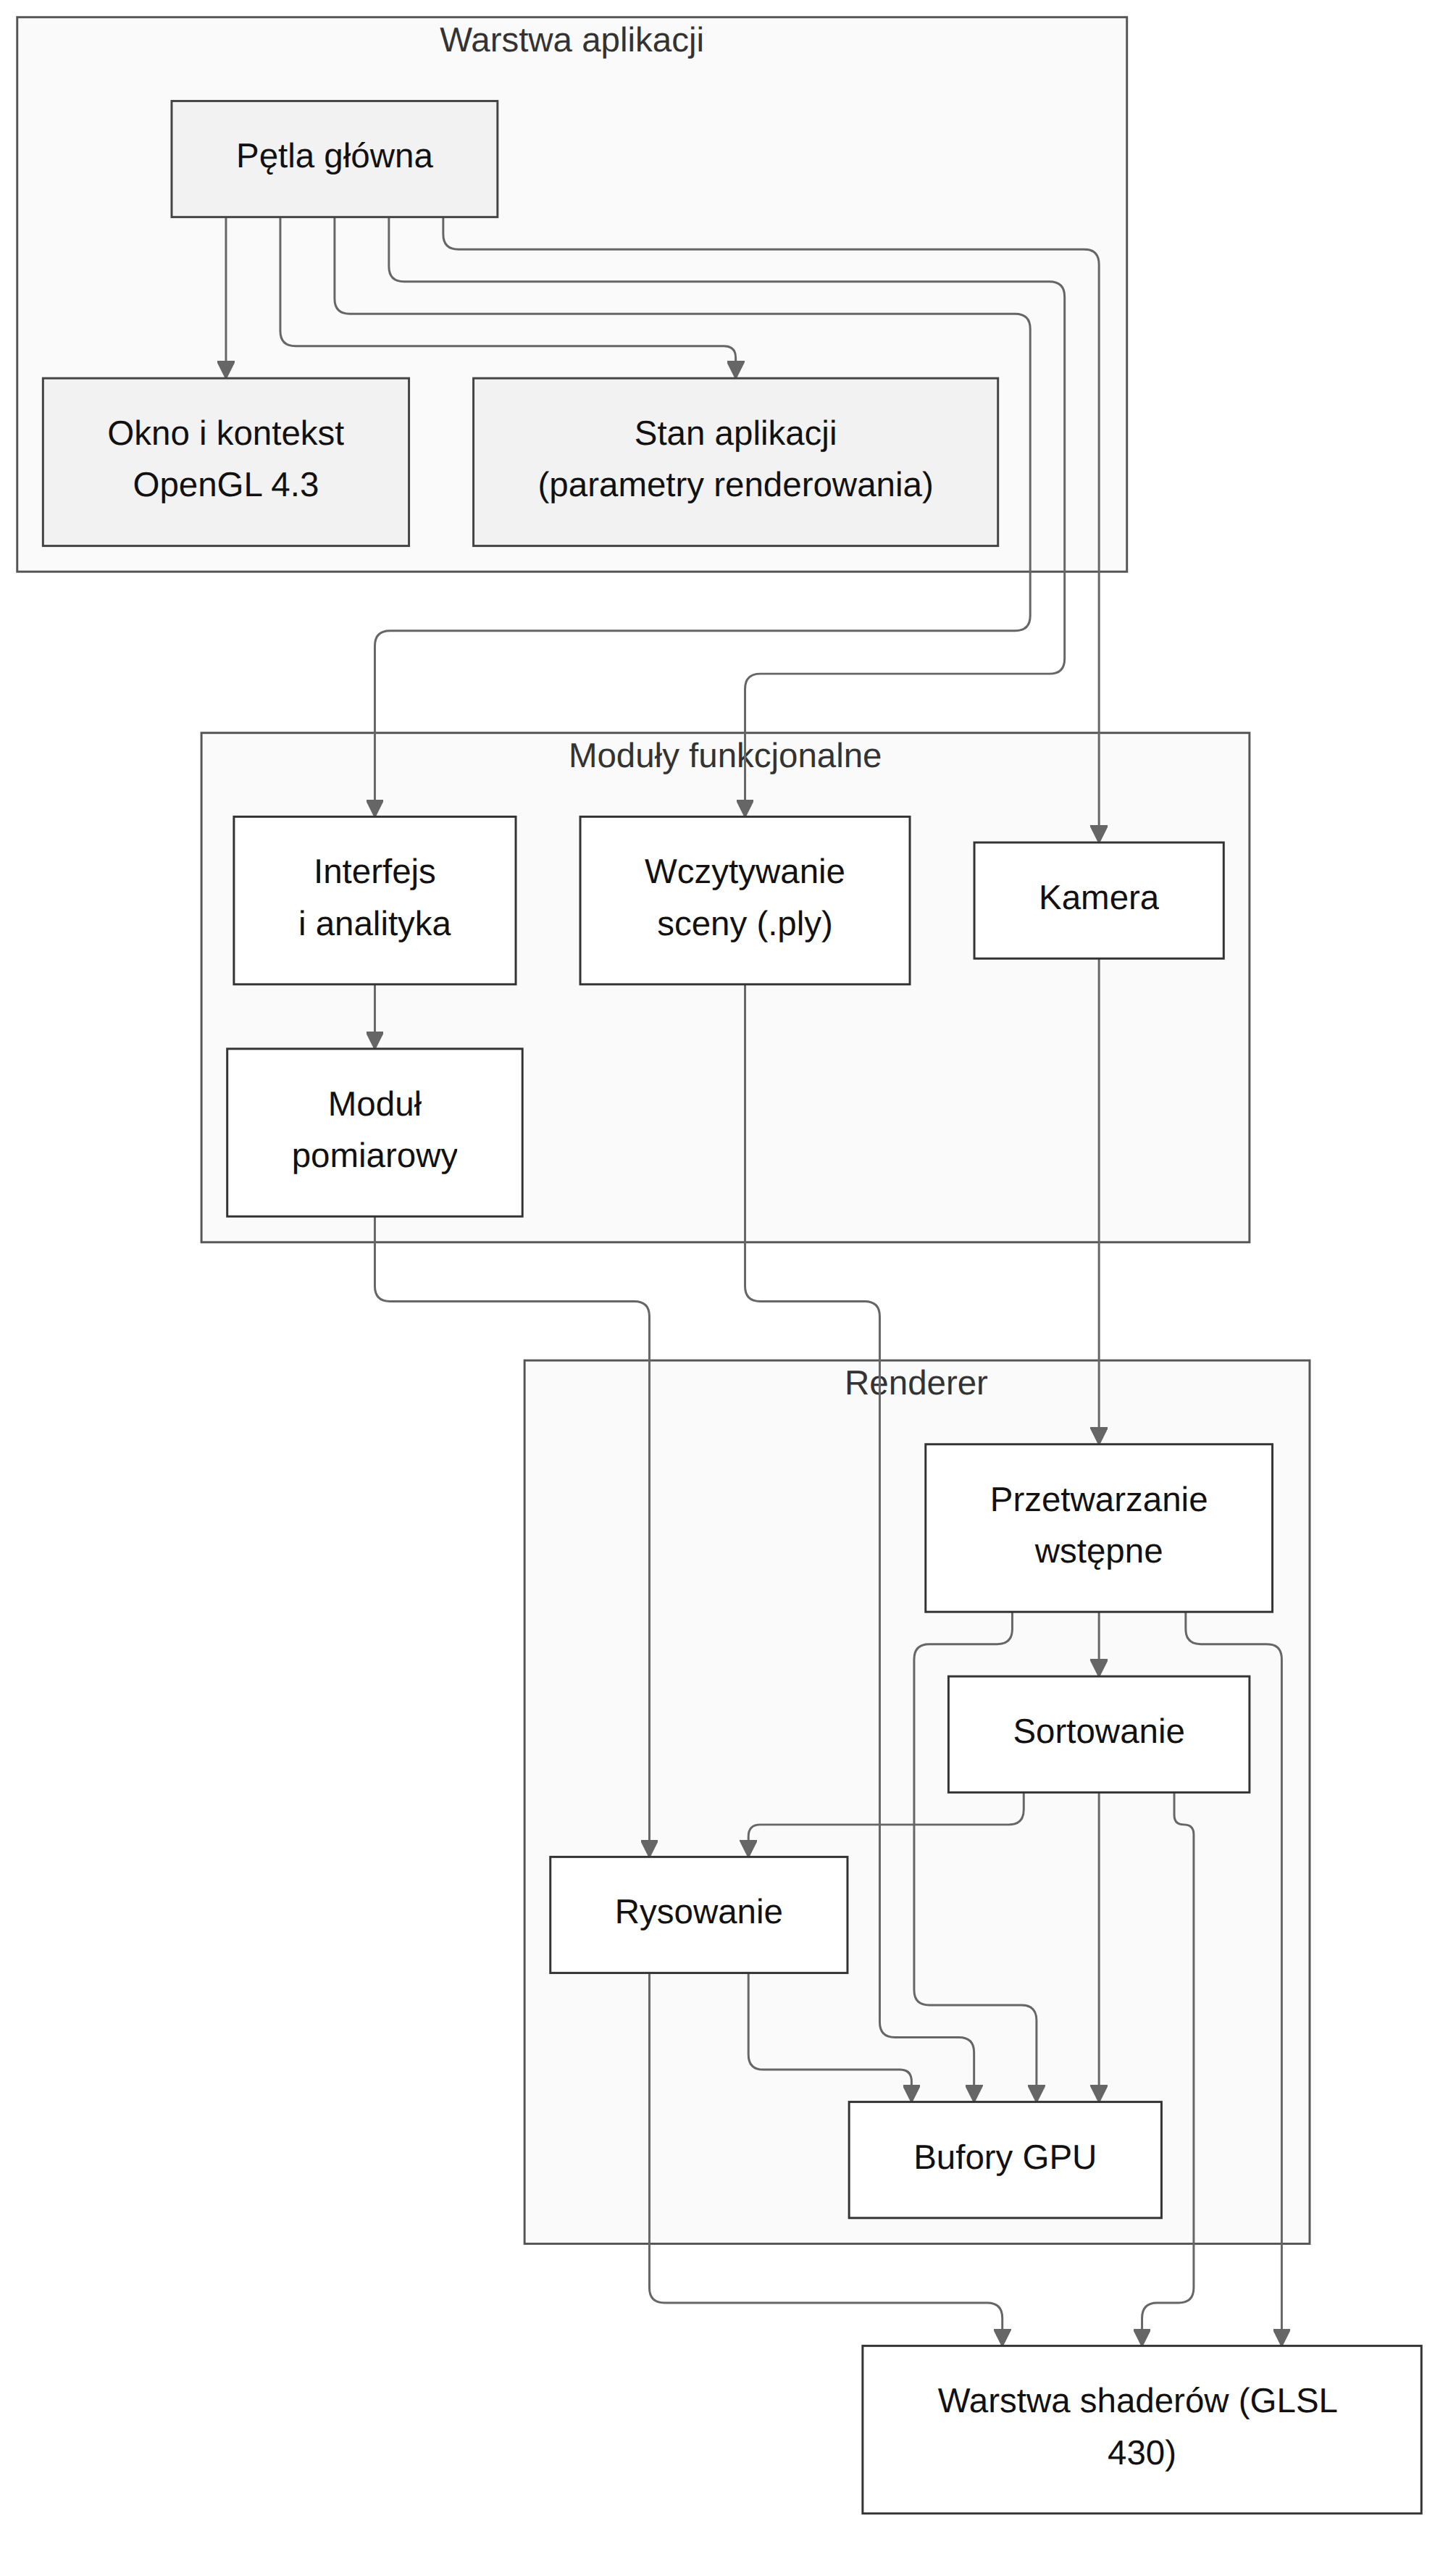
\includegraphics[width=0.8\textwidth]{rys_komponenty}
  \caption{Diagram komponentów systemu; strzałki oznaczają kierunek zależności}
  \label{rys:komponenty}
\end{figure}

\section{Model danych}
\label{sec:model}
\subsection{Reprezentacja splatu w pamięci}
\label{subsec:struktura}
Pojedyńczy Gaussian został opisany strukturą w C++. Jest to struktura o stałym rozmiarze, zawierająca 59 liczb zmiennoprzecinkowych co daje 236 bajtów na splat. Układ pół przedstawia poniższa tabela \ref{tab:splat}.
\begin{table}[htbp]
  \centering
  \caption{Układ pól struktury opisującej pojedynczy splat}
  \label{tab:splat}
  \small
  \renewcommand{\arraystretch}{1.15}
  \begin{tabularx}{\textwidth}{
      >{\raggedright\arraybackslash}p{0.2\textwidth}
      >{\centering\arraybackslash}p{0.11\textwidth}
      >{\centering\arraybackslash}p{0.11\textwidth}
      >{\raggedright\arraybackslash}X}
    \toprule
    \textbf{Pole} & \textbf{Liczby} & \textbf{Bajty} & \textbf{Znaczenie} \\
    \midrule
    Pozycja        & 3  & 12  & środek Gaussiana w przestrzeni sceny \\
    Składowa DC    & 3  & 12  & barwa niezależna od kierunku patrzenia \\
    Nieprzezroczystość & 1  & 4   & wartość $\alpha$ po funkcji sigmoidalnej \\
    Skala          & 3  & 12  & odchylenia wzdłuż osi własnych elipsoidy \\
    Kwaternion     & 4  & 16  & orientacja elipsoidy \\
    Pozostałe SH   & 45 & 180 & współczynniki pasm 1--3 harmonik sferycznych \\
    \midrule
    \textbf{Razem} & \textbf{59} & \textbf{236} & \\
    \bottomrule
  \end{tabularx}
\end{table}
\subsection{Podział pamięci między procesor a kartę graficzną}
\label{gpudata}
Każda scena istnieje w dwóch kopiach: w pamięci operacyjnej, gdzie jest wykorzysytwana do sortowania na CPU i analizie danych, oraz w pamięci karty graficznej, gdzie jest źródłem danych dla wszystkich etapów potoku graficznego. W projekcie występuje jedenaście buforów typu SSBO, przypisanych do stałych punktów dowiązania (tabela \ref{tab:bufory})
\begin{table}[htbp]
  \centering
  \caption{Bufory danych w pamięci karty graficznej}
  \label{tab:bufory}
  \small
  \renewcommand{\arraystretch}{1.15}
  \begin{tabularx}{\textwidth}{
      >{\raggedright\arraybackslash}p{0.26\textwidth}
      >{\raggedright\arraybackslash}p{0.16\textwidth}
      >{\raggedright\arraybackslash}X}
    \toprule
    \textbf{Bufor} & \textbf{Rozmiar} & \textbf{Rola} \\
    \midrule
    Splaty & $236N$ B & niezmienna kopia sceny \\
    Wyniki przetwarzania & $48N$ B & rzutowany środek, odwrócona kowariancja
      2D, barwa, rozmiar ekranowy \\
    Indeksy rysowania & $4N$ B & kolejność kompozycji \\
    Indeksy widoczne & $4N$ B & lista splatów po odrzuceniu \\
    Licznik widocznych & 4 B & wynik kompaktowania \\
    Klucze A i B & $2\times4N$ B & klucze sortowania (bufory zamieniane
      w kolejnych przebiegach) \\
    Indeksy B & $4N$ B & bufor docelowy przestawiania \\
    Histogramy grup & $64W$ B & liczności cyfr w grupach roboczych \\
    Przesunięcia kubełków & 64 B & wynik sumowania prefiksowego \\
    Licznik fragmentów & 4 B & pomiar przerysowania \\
    \bottomrule
  \end{tabularx}
\end{table}
Oznaczając przez $N$ liczbę spatów, a przez $W$ liczbę grup roboczych możemy oszacować całkowite zapotrzebowanie na pamięć karty graficznej (VRAM) przez wzór
\begin{equation}
    M(N) = 304\,N + 64\,W + \mathcal{0}(1) \ \ \text{[B]},
    \label{eq:pamiec}
\end{equation}
Wychodzi to około 304 bajty na splat. Dla sceny miliona Gaussianów daje to w przybliżeniu 290 MiB, a dla sceny sześciomilionowej blisko 1,7 GiB. Stąd pojawia się wymaganie WN-04: użytkownik powinien poznać skalę zapotrzebowania przed próbą wczytania sceny której karta nie pomieści.

\section{Projekt potoku renderowania}
\label{sec:pipeline}
\subsection{Przebieg pojedynczej klatki}
\label{subsec:klatka}
Potok zaprojektowano jako sekwencję sześciu etapów, z których dwa są warunkowe (rysunek \ref{rys:przeplyw}).
\begin{enumerate}
    \item \textbf{Obsługa wejścia i aktualizacja kamery.} Akcje myszy przeliczane są na zmianę kątów, punktu docelowego lub promienia. Macierz widoku jest przeliczana leniwie - wyłącznie wtedy, gdy któryś z paramertów uległ zmianie.
    \item \textbf{Przetwarzanie wstępne.} Dla każdego splatu wyznaczane są: macierz kowariancji 3D z rozkładu na skalę i rotację, jej rzut na płaszczyznę ekranu, barwa z harmonik sferycznych dla bieżącego kierunku patrzenia, głębokość oraz rozmiar elipsy w pikselach. Na tym samym etapie zostają odrzucone  splaty poza polem widzenia i poniżej progu przeźroczystości, a te które zostaną, są dodawane do ciągłej listy indeksów.
    \item \textbf{Sortowanie.} Widoczne splaty są porządkowane w porządku malejącym ze względu na głębokość. Sortowanie następuje tylko wtedy gdy zmienimy pozycję w scenie jedną z dwóch metod opisanych w podrozdziale 3.6.2.
    \item \textbf{Rysowanie.} Wykorzystując instancing sprzętowy  powielamy pojedynczy czworobok tyle razy, ile jest splatów widocznych. Program wierzchołków \eng{Vertex Shader} rozciąga czworobok do rozmiaru elipsy, a program fragmentów \eng{Fragment Shader} wyznacza wartość gęstości Gaussiana w pikselu i wynikowe krycie.
    \item \textbf{Kompozycja.} Fragmenty są mieszane operatorem "over" z krycia przemnożonego, przy wyłączonym teście głębokości.
    \item \textbf{Interfejs i analityka.} Panel sterowania oraz wykresy są rysowane na wierzchu obrazu sceny w tym samym kontekście OpenGL.
\end{enumerate}
\begin{figure}[htbp]
  \centering
  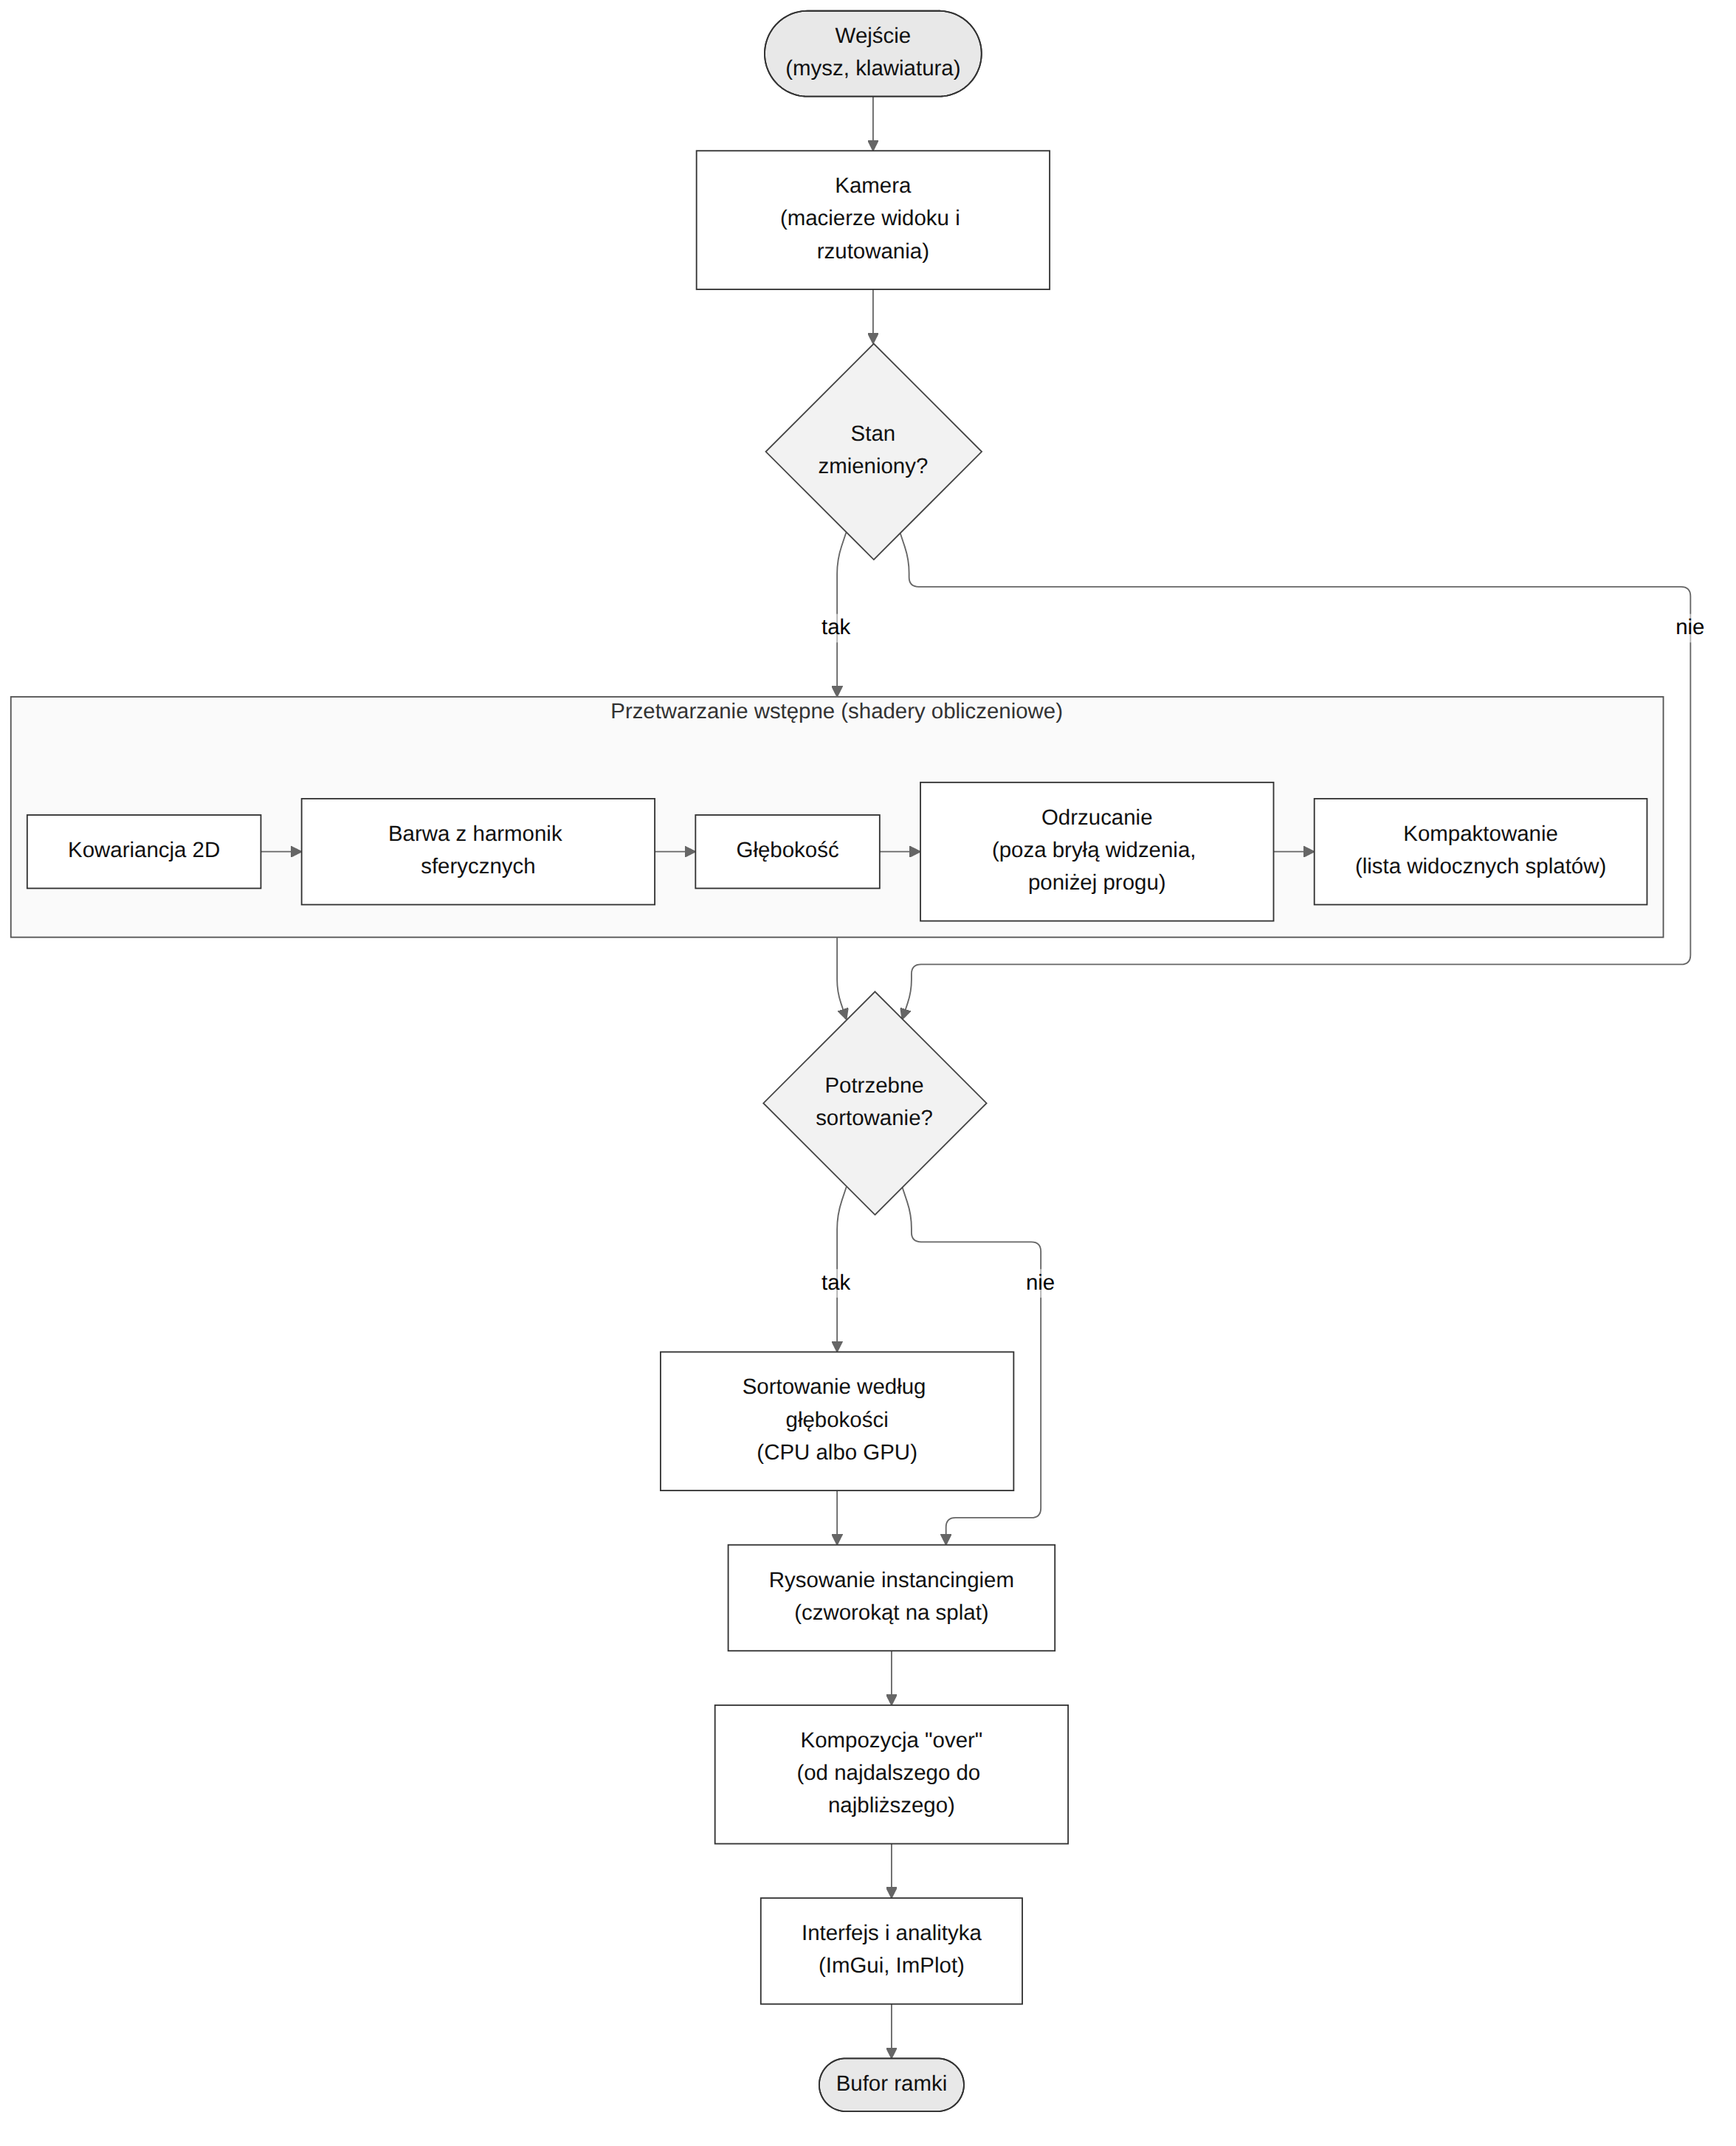
\includegraphics[width=0.95\textwidth]{rys_przeplyw}
  \caption{Przepływ danych podczas renderowania pojedynczej klatki}
  \label{rys:przeplyw}
\end{figure}
Istotnym elementem projektu jest warunkowość etapów 2 i 3. Wyniki przetwarzania wstępnego zależą wyłącznie od macierzy widoku, projekcji, położenia kamery, rozmiaru okna oraz zestawu parametrów renderowania. Jeśli żadna z tych wartości się nie zmieni, otrzymamy ten sam wynik. Analogicznie to działa dla etapu sortowania: dopóty, dopóki kamera nie przemieści się na tyle, by zmieniła się głębokość splatów. Należy wspomnić że ponowne sortowanie wyzwalane jest tylko, gdy obserwator (kamera) przesunie się o więcej niż 0,2\% bieżącego promienia orbity, stąd wynika, że próg ten jest proporcjonalny do promienia, a nie jest stały.

\subsection{Projekt dwóch ścieżek sortowania}
\label{subsec:sortowanie}
Kompozycja Gaussianów jest operacją zależną od kolejności dlatego tak istotne jest zaimplementowanie wydajnego sortowania. W projekcie zaimplementowane są dwie ścieżki, między którymi można się przełączać w czasie działania programu:
\begin{itemize}
    \item \textbf{ścieżka CPU} - sortowanie przez porównania biblioteki standardowej wykonywane na tablicy indeksów i tablicy głębokości w pamięci RAM.
    \item \textbf{ścieżka GPU} - sortowanie pozycyjne \eng{radix sort} w wariancie od najmłodszej cyfry, zrealizowane w czterech shaderach obliczeniowych (wyznaczanie kluczy, histogram, sumowanie prefiksowe \eng{prefix sum}, przestawianie) i przebiegające bez opuszczania VRAM (wszystkie dane są od początku w pamięci karty graficznej)
\end{itemize}
Ścieżka GPU zawsze jest bardziej wydajna niż na CPU, jednak została ona zachowana, żeby można było porównać wydajność tych dwóch podejść. Sortowanie na CPU było łatwiejsze w implementacji, jednak różnica czasu przemawia na korzyść sortowania na GPU. Możliwość przełączania istnieje w aplikacji bez potrzeby ponownego uruchamiania aplikacji, co sprawia, że oba warianty porównywane są w tym samym środowisku.
Kluczem sortowania jest 32-bitowa liczba całkowita wyprowadzona z głębokości splatu w przestrzeni kamery. Dzięki odwzorowaniu zachowującemu porządek, porównywanie kluczy całkowitych da ten sam wynik co porównywanie liczb zmiennoprzecinkowych, lecz w kolejności od najdalszego do najbliższego. Sortowanie pozycyjne z natury porządkuje liczby rosnąco i operuje na liczbach bez znaku, co sprawia, że nie musimy użyć dodatkowego przebiegu odwracającego wynik. Zostały przyjęte cyfry czterobitowe, co daje szesnaście kubełków i osiem przebiegów na pełny klucz.
\subsection{Decyzja o modelu rasteryzacji}
\label{subsec:raster}
W zaprojektowanym systemie przyjęto, że każdy splat generuje własny czworobok, opisując jego elipsę, a sortowanie jest globalne. Jest to różnica między implementacją oryginalną, gdzie ekran jest podzielony na kafle i dla każdego kafla buduje się listę przecinających go Gaussianów, które są sortowane lokalnie. Podejście przedstawione w tym projekcie jest łatwiejsze i wpisuje się w sprzętowy potok rasteryzacji, nie wymaga budowania struktur pośrednich i nie wymaga mechanizmów, których OpenGL 4.3 Core nie udostępnia w wygodnej postaci.
Kosztem takiej decyzji jest przerysowanie: fragmenty odrzucane w programie fragmentów są mimo wszystko rasteryzowane. Ponieważ jest to główne ograniczenie przyjętego modelu, stworzono dwa mechanizmy pozwalające je zmierzyć(WF-08, WF-11). Parametr maksymalnego promienia splatu (WF-07) pozwala z kolei ograniczyć wpływ bardzo dużych elips.
\section{Projekt interfejsu użytkownika}
\label{sec:gui}
Interfejs został zbudowany jako jeden panel złożony z pięciu zwijanych sekcji co odpowiada wymaganiu WN-09. Każda z sekcji mówi o czymś innym:
\begin{itemize}
    \item \textbf{Scena} - zawiera nazwę pliku, liczbę splatów, szacowane zajęcie pamięci karty graficznej, przycisk wyboru pliku, komunikat o błędzie wczytywania, przycisk do zrzutu ekranu.
    \item \textbf{Ustawienia kamery} - zapis, przywracanie i usuwanie nazwanych ustawień.
    \item \textbf{Renderowanie} - zawiera suwaki parametrów potoku renderowania wraz z podpowiedziami.
    \item \textbf{Widok} - Wybór trybu wizualizacji oraz przełącznik podzielonego ekranu.
    \item \textbf{Statystyki} - licznik czasu, wybór metody sortowania, przyciski testów poprawności.
    \item \textbf{Analiza} - histogramy właściwości widocznych splatów.
\end{itemize}
Histogramy dotyczą tylko tych splatów, które są aktualnie widoczne, a więc zbioru zmieniającego się z każdym ruchem kamery. Przeliczanie setki parametrów w każdej klatce obciążyłoby system. Żeby temu zaradzić użytkownik sam decyduje, kiedy pobrać dane z karty graficznej i przeliczyć rozkłady. Wykres historii liczby klatek na sekundę pozostaje ciągły.
Sterowanie kamerą orbitalną oparto na trzech gestach myszy - przeciąganie lewym przyciskiem (obracanie), przeciąganie prawym przyciskiem (przesuwanie) i obracanie kółkiem (przybliżanie). Przybliżanie jest proporcjonalne do bieżącej odległości od sceny, co daje podobny efekt wizualny niezależnie od tego, czy obserwator ogląda scenę z dystansu, czy bada jej fragment z bliska.

\section{Projekt modułu pomiarowego}
\label{sec:measure}
Wymaganie WN-05 (powtarzalność pomiarów) nie daje się spełnić w trybie interaktywnym: wyniki jakie otrzymamy przy ręcznym poruszaniu kamerą nie są porównywalne między wariantami potoku, ponieważ nie da się powtórzyć tej samej trajektorii. Zaprojektowano więc mechanizm uruchamiany z wiersza poleceń oparty na trzech elementach. 

Pierwszym jest deterministyczna trajektori kamery, zapisana w pliku tekstowym jako ciąg klatek pośrednich. Położenie obserwatora w klatce pośredniej powstaje poprzez interpolację między sąsiednimi klatkami kluczowymi. Ten sam plik da za każdym razem tę samą sekwencję widoków.

Drugim jest pomiar czasu po stronie GPU. Czas mierzony zegarem procesora obejmowałby tylko czas zlecenia pracy, a nie jej wykonania, bo zadania graficzne są wykonywane asynchronicznie. Zaprojektowano pomiar oparty na zapytaniach karty graficznej, z jawną synchronizacją na końcu klatki w trybie wsadowym oraz z odczytem opóźnionym w trybie interaktywnym.

Trzecim jest \textbf{raport w formacie CSV}: jeden wiersz na klatkę,
zawierający numer klatki, czas całkowity, czas sortowania, czas pracy karty
graficznej, liczbę splatów widocznych oraz liczbę wygenerowanych fragmentów,
a na końcu wiersze podsumowania z wartością średnią, medianą i percentylem
99. Wybór formatu tekstowego jest celowy  -  wyniki trafiają wprost do
narzędzia arkuszowego, a plik pozostaje czytelny w postaci źródłowej.
 
Oddzielnym zagadnieniem jest weryfikacja \textbf{poprawności wizualnej}.
Ponieważ system jest samodzielną implementacją metody opisanej w oryginalnej pracy, potrzebna jest miara odchylenia od obrazu odniesienia.
Zaprojektowano tryb porównania dwóch obrazów, wyznaczający szczytowy stosunek
sygnału do szumu \eng{peak signal-to-noise ratio} oraz wskaźnik podobieństwa
strukturalnego \eng{structural similarity index}. Pierwsza miara wykrywa
różnice punktowe, druga  -  różnice w strukturze obrazu, bliższe percepcji
obserwatora. W połączeniu ze zrzutem klatki o zadanym numerze, wykonywanym
w trybie wsadowym, pozwala to porównywać obrazy pochodzące dokładnie z tej
samej pozycji kamery.
 
\section{Zestawienie decyzji projektowych}
\label{sec:decyzje}
 
Tabela \ref{tab:decyzje} zbiera najważniejsze decyzje podjęte na etapie
projektowania wraz z rozważaną alternatywą i ceną, jaką za każdą z nich
zapłacono. Jawne wskazanie kosztu jest tu równie istotne jak uzasadnienie:
każda z tych decyzji zawęża możliwości systemu w konkretny, dający się
wskazać sposób.
 
\begin{table}[htbp]
  \centering
  \caption{Kluczowe decyzje projektowe}
  \label{tab:decyzje}
  \small
  \renewcommand{\arraystretch}{1.15}
  \begin{tabularx}{\textwidth}{
      >{\raggedright\arraybackslash}p{0.2\textwidth}
      >{\raggedright\arraybackslash}X
      >{\raggedright\arraybackslash}X}
    \toprule
    \textbf{Decyzja} & \textbf{Uzasadnienie} & \textbf{Koszt} \\
    \midrule
    Billboardy z instancingiem zamiast rasteryzacji kafelkowej &
      Bezpośrednie wykorzystanie sprzętowego potoku rasteryzacji, brak
      struktur pośrednich, realizowalne w rdzeniu OpenGL 4.3 &
      Przerysowanie rosnące z rozmiarem elips; brak przycinania splatów do
      kafli \\
    Sortowanie globalne zamiast lokalnego w kaflach &
      Jeden porządek dla całej sceny, prostsza weryfikacja poprawności &
      Sortowany jest cały zbiór widoczny, także gdy zmiana dotyczy
      fragmentu obrazu \\
    Dwie współistniejące ścieżki sortowania &
      Wariant procesorowy jako wzorzec poprawności, różnica czasów jako
      materiał pomiarowy &
      Podwojony kod ścieżki sortowania i dodatkowe bufory \\
    Przetwarzanie wstępne na karcie graficznej &
      Zrównoleglenie operacji wykonywanej dla każdego splatu; uniknięcie
      przesyłania wyników przez magistralę &
      Trudniejsze diagnozowanie błędów niż w kodzie procesora \\
    Odczyt liczby splatów widocznych do pamięci operacyjnej &
      Umożliwia sterowanie rysowaniem i analitykę po stronie procesora &
      Synchronizacja potoku przy każdym ruchu kamery \\
    Kamera wyłącznie orbitalna &
      Zgodność z konwencją narzędzi do oglądania obiektów; prostsze
      i odporniejsze sterowanie &
      Brak swobodnego przelotu przez wnętrze sceny \\
    Aplikacja jednowątkowa po stronie procesora &
      Praca warta zrównoleglenia trafia na kartę graficzną; brak klasy
      błędów synchronizacji &
      Wczytywanie sceny blokuje interfejs \\
    Wyłącznie format \texttt{.ply} &
      Zgodność z implementacją referencyjną, brak warstwy dekompresji &
      Brak obsługi formatów skompresowanych, większe pliki wejściowe \\
    \bottomrule
  \end{tabularx}
\end{table}
 
\section{Podsumowanie rozdziału}
\label{sec:podsumowanie3}
 
W rozdziale przedstawiono projekt systemu wizualizacji scen 3DGS:
szesnaście wymagań funkcjonalnych i dziewięć pozafunkcjonalnych, podział na
siedem modułów o jednokierunkowych zależnościach, model danych oparty na
strukturze 236 bajtów na splat i jedenastu buforach karty graficznej,
sześcioetapowy potok renderowania z dwoma etapami warunkowymi oraz projekt
warstwy pomiarowej zapewniającej powtarzalność wyników.
 
Przyjęte rozwiązania wynikają wprost z luki wskazanej w rozdziale
pierwszym. Niezależność od CUDA jest konsekwencją oparcia całego potoku na
rdzeniu OpenGL 4.3 (WN-01); warstwa analityczna, której brakuje narzędziom
spoza ekosystemu NVIDIA, została zaprojektowana jako zestaw wymagań
WF-08--WF-11; ergonomia, słaba strona narzędzi analitycznych, jest
przedmiotem wymagania WN-09 i projektu interfejsu z podrozdziału \ref{sec:gui}.
 
Sposób realizacji poszczególnych wymagań  -  struktury danych, programy
shaderowe i algorytmy  -  opisano w rozdziale następnym. Weryfikację
wymagań wydajnościowych oraz poprawności wizualnej, wykonaną narzędziami
zaprojektowanymi w podrozdziale \ref{sec:measure}, przedstawiono
w rozdziale poświęconym wynikom testów.

\printbibliography[heading=bibintoc, title={Bibliografia}]

\end{document}
